%%% common LaTeX classes will work fine
\documentclass[oneside,11pt]{amsart}

%%% recommended for PDF quality: better handling of accented characters and ligatures
\usepackage[utf8]{inputenc}
\usepackage[T1]{fontenc}

%%% REQUIRED for accessibility: set the language for the output (here 'en-GB')
\usepackage[british]{babel}

%%% REQUIRED for correct formatting and tagging of BookML output: title and author
\title{Lecture 1: Foundations in Deterministic and Stochastic Optimization}
\author{Stefan Vlaski and Ali H. Sayed}
\date{}

%%% RECOMMENDED for PDF quality: enable clickable links and metadata in PDFs
% the option pdfusetitle adds \author and \title to the PDF metadata
\usepackage[pdfusetitle]{hyperref}

%%% RECOMMENDED for PDF quality: higher quality equivalent of Computer Modern
\usepackage{lmodern}

%%% OPTIONAL: additional BookML and LaTeXML functionality
\usepackage{bookml/bookml}

%%% REQUIRED for TikZ: use bmlImageEnvironment for TikZ and other images, since
%%%                    LaTeXML is slow and often produces garbled TikZ output
%%%                    (this requires \usepackage{bookml/bookml})
% tell BookML to compile tikzpicture and tikzcd environments into images via LaTeX
\bmlImageEnvironment{tikzpicture,tikzcd}
% hide all TikZ-related commands from LaTeXML, but leave them when generating the PDF
\iflatexml            % are we compiling through LaTeXML?
\else
\usepackage{tikz}     % if not, load TikZ as usual
\usetikzlibrary{cd}
\usepackage[all]{xy}
% other TikZ-related command MUST be here, before \fi
\fi

%%% OPTIONAL for accessibility: additional versions of the document (e.g. large print)
% the additional formats will be recompiled automatically whenever there are changes
% you may use "\jobname" instead of "template" to pick up the name from this very file
\bmlAltFormat{lecture1.pdf}{PDF (serif)} % always included; here \bmlAltFormat simply changes its label
%\bmlAltFormat{template-sans.pdf}{PDF (sans serif)}
%\bmlAltFormat{template-sans-large.pdf}{PDF (sans, large)}

% very cheap way of generating a 'large print' PDF (~19% bigger)
\ifcsname bmlCrop\endcsname % is \bmlCrop defined?
\usepackage{crop}           % if so, load the package crop
\fi
%%% What is \bmlCrop?
% template-sans-large.tex uses \input{template.tex} to read this file.
% Before that, it defines \bmlCrop, so that the above code imports crop.
% It also uses \PassOptionsToPackage to tweak the options of crop.
% The result has identical pagination as the normal PDF so you do not need
% to review both versions.
%
% However, the magnification is very limited. If you need larger magnification,
% you may have to use a larger font, in which case the large print PDF will
% will look different and must be reviewed regularly.

% rest of preamble



\def\A{{\boldsymbol{A}}}
\def\B{{\boldsymbol{B}}}
\def\C{{\boldsymbol{C}}}
\def\D{{\boldsymbol{D}}}
\def\E{{\boldsymbol{E}}}
\def\F{{\boldsymbol{F}}}
\def\G{{\boldsymbol{G}}}
\def\H{{\boldsymbol{H}}}
\def\I{{\boldsymbol{I}}}
\def\J{{\boldsymbol{J}}}
\def\K{{\boldsymbol{K}}}
\def\L{{\boldsymbol{L}}}
\def\M{{\boldsymbol{M}}}
\def\N{{\boldsymbol{N}}}
\def\O{{\boldsymbol{O}}}
\def\P{{\boldsymbol{P}}}
\def\Q{{\boldsymbol{Q}}}
\def\R{{\boldsymbol{R}}}
\def\S{{\boldsymbol{S}}}
\def\T{{\boldsymbol{T}}}
\def\U{{\boldsymbol{U}}}
\def\V{{\boldsymbol{V}}}
\def\W{{\boldsymbol{W}}}
\def\X{{\boldsymbol{X}}}
\def\Y{{\boldsymbol{Y}}}
\def\Z{{\boldsymbol{Z}}}

\def\a{{\boldsymbol{a}}}
\def\b{{\boldsymbol{b}}}
\def\c{{\boldsymbol{c}}}
\def\d{{\boldsymbol{d}}}
\def\e{{\boldsymbol{e}}}
\def\f{{\boldsymbol{f}}}
\def\g{{\boldsymbol{g}}}
\def\h{{\boldsymbol{h}}}
\def\j{{\boldsymbol{j}}}
\def\k{{\boldsymbol{k}}}
\def\l{{\boldsymbol{l}}}
\def\m{{\boldsymbol{m}}}
\def\n{{\boldsymbol{n}}}
\def\o{{\boldsymbol{o}}}
\def\p{{\boldsymbol{p}}}
\def\q{{\boldsymbol{q}}}
\def\r{{\boldsymbol{r}}}
\def\s{{\boldsymbol{s}}}
\def\t{{\boldsymbol{t}}}
\def\u{{\boldsymbol{u}}}
\def\v{{\boldsymbol{v}}}
\def\w{{\boldsymbol{w}}}
\def\x{{\boldsymbol{x}}}
\def\y{{\boldsymbol{y}}}
\def\z{{\boldsymbol{z}}}

\theoremstyle{remark}
\newtheorem{remark}{Remark}[section]

\usepackage{amsmath}
\usepackage{amsthm}
\usepackage{amssymb}
\usepackage{graphicx}
\usepackage{dsfont}

\begin{document}

%%% RECOMMENDED for SCORM: the abstract becomes the description of the SCORM package
\begin{abstract}
  These notes cover foundational material in statistical learning theory as well as deterministic and stochastic optimization with a focus on single agent learners. It is expected that the reader will have had some exposure to concepts such as maximum likelihood and maximum a posteriori estimation, gradient descent as well as its stochastic variants, and as a result the exposition is kept brief. Nevertheless, we find it useful to collect this information here as it will form the foundation for the development of multi-agent learning algorithms in future lectures.
\end{abstract}

\maketitle

%%% OPTIONAL: footer for HTML output, for instance a copyright notice
% note that the footer does not appear in the PDF
% the PDF footer can be done in any of the usual ways (e.g. fancyhdr)
\begin{lxFooter}
  \copyright\ 2024. All rights reserved. These notes cannot be copied or distributed in print or electronically without the written consent of the authors S. Vlaski and A. H. Sayed.
\end{lxFooter}

\section{Baysian Inference}
One of the most fundamental problems in statistics, signal processing, and machine learning, is the \emph{inference} problem, where we wish to construct an estimate of some random quantity of interest \( \boldsymbol{\gamma} \in \mathds{R}^{M_{\boldsymbol{\gamma}}}\), given observations of a related random variable \( \boldsymbol{h} \in \mathds{R}^{M_{\boldsymbol{h}}} \). The quantity of interest \( \boldsymbol{\gamma} \) may take on continuous or discrete values, and is referred to as the ``dependent variable,'' ``state of nature,'' ``class,'' or ``label'' depending on the application. We will most commonly refer to it as the label. We will refer to the observed random variable \( \boldsymbol{h} \) generally as the feature, although in some applications it is known as ``regressor'' or ``observation''.

If we are provided with the conditional distribution \( f_{\boldsymbol{\gamma}|\boldsymbol{h}}(\gamma | h) \) along with a single realization of the feature \( \boldsymbol{h} \), it is quite natural to estimate \( \boldsymbol{\gamma} \) as the most likely outcome given \( \boldsymbol{h} \). We can express this formally as:
\begin{align}\label{eq:baysian_framework}
  {\gamma^{\star}} \triangleq \arg\max_{{\gamma} \in \Gamma} f_{\boldsymbol{\gamma}|\boldsymbol{h}}(\gamma | h)
\end{align}
The conditional distribution \( f_{\boldsymbol{\gamma}|\boldsymbol{h}}(\gamma | h) \) is frequently referred to as the \emph{posterior distribution} of \( \boldsymbol{\gamma} \), making \( {\gamma^{\star}} \) the \emph{maximum a posteriori (MAP) estimate} of \( \boldsymbol{\gamma} \) given \( \boldsymbol{h} \). We note that it is common in the literature on estimation theory to the employ hat-notation to refer to estimates of a random quantity based on data. In this sense, we could have opted to denote the optimal solution to~\eqref{eq:baysian_framework} by \( \widehat{\gamma} \), rather than \( \gamma^{\star} \). Nevertheless, as we transition from inference to learning and optimization, we will increasingly interpret estimates as solutions to generic optimization problems. In this context, it will be appropriate to employ the \( ^{\star} \)-notation to refer to an optimal solution. To preserve consistency throughout this text, we opt to use the \( ^{\star} \)-notation from the onset, with the understanding that within the Bayesian framework~\eqref{eq:baysian_framework} the optimal solution \( \gamma^{\star} \) carries the interpretation of an estimate. Finally, we note that~\eqref{eq:baysian_framework} is formulated for a particular realization \( h \) of the random variable \( \boldsymbol{h} \). As we will see, most MAP estimators are derived for a particular realization of the feature vector, resulting in a deterministic estimate \( \gamma^{\star} \) as a function of the realization \( h \). We can also regard the MAP solution as a random variable, denoted in boldface notation $\boldsymbol{\gamma}^{\star}$, when it is viewed as a function of the random observation \( \h\):
\begin{align}
  \boldsymbol{\gamma}^{\star} \triangleq \arg\max_{{\gamma} \in \Gamma} f_{\boldsymbol{\gamma}|\boldsymbol{h}}(\gamma | \boldsymbol{h})
\end{align}
where the posterior distribution \( f_{\boldsymbol{\gamma}|\boldsymbol{h}}(\gamma | \boldsymbol{h}) \) is now a function of the random variable \( \boldsymbol{h} \), rather than its realization \( h \).
{\begin{remark}[\textbf{ Bold font indicates random variables}] We note that we employ bold font to denote a random variables, for example \( \boldsymbol{h} \), while regular font denotes its realization or a deterministic quanity, as in \( h \). As a general rule, we use lowercase fonts to denote vectors, while uppercase letters denote matrices. In this way, a random matrix would be denoted by \( \boldsymbol{H} \), while its realization would correspond to \( H \).
\end{remark}
}

\begin{figure}[h]
	\begin{center}
		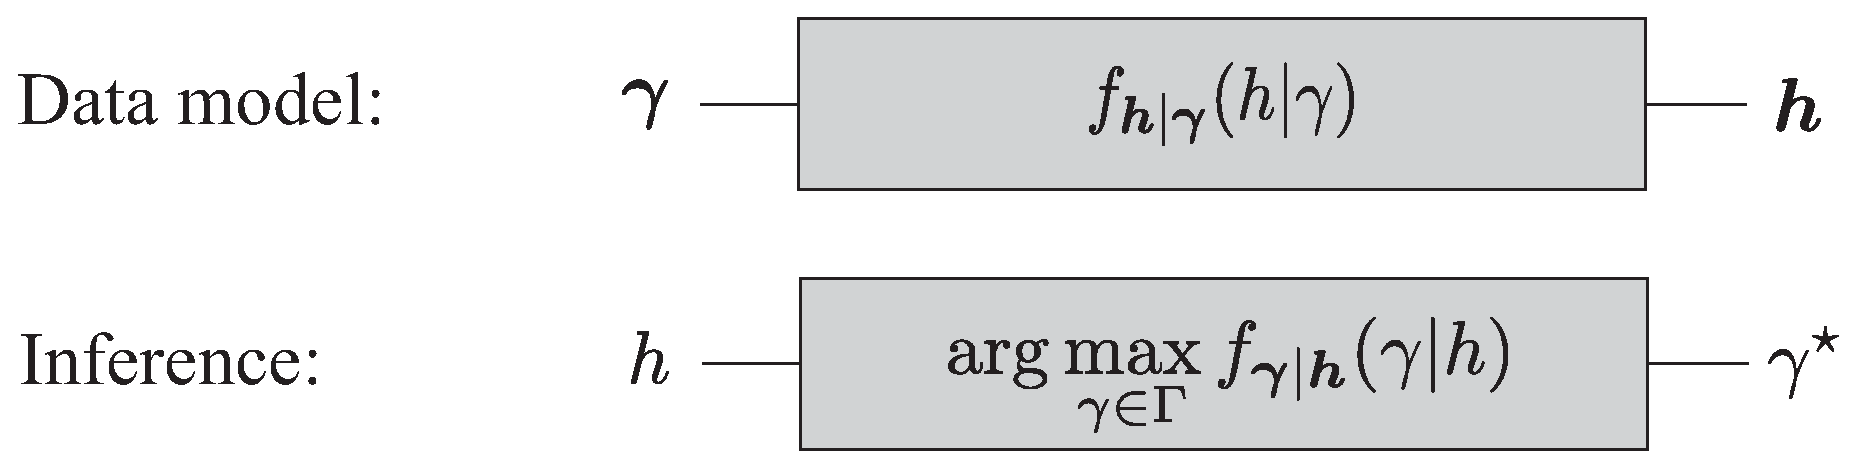
\includegraphics[width=.6\textwidth]{Inference_Fig1_new.eps}
		\caption{{\small A general model underlying most inference problems. The top row illustrates the generative model for the observations $\h$, while the bottom row illustrates the Bayesian inference formulation for recovering the label variable.}}
		\label{fig:ch_inference_fig1}
	\end{center}
\end{figure}

\section{From Inference to Learning}
Our previous discussion leading has uncovered how to perform MAP inference of a random quantity of interest \( \boldsymbol{\gamma} \) given observations \( \{ \boldsymbol{h}_n \}_{n=1}^N \), models \( f_{\boldsymbol{h} | \boldsymbol{\gamma} } \left( \cdot | {\gamma} \right) \), and prior information \( f_{\boldsymbol{\gamma}}(\gamma) \). In many practical situations, we are not provided with prior knowledge about the model relating the label \( \boldsymbol{\gamma} \) with the feature \( \boldsymbol{h} \). Instead, we need to estimate \( f_{\boldsymbol{h} | \boldsymbol{\gamma} } \left( \cdot | {\gamma} \right) \) from data before performing inference. We refer to the process of estimating statistical properties of data needed for inference, such as \( f_{\boldsymbol{h} | \boldsymbol{\gamma} } \left( \cdot | {\gamma} \right) \), as \emph{learning}. As we will see in this section, the learning of models can be formalized using a Bayesian MAP framework analogous to~\eqref{eq:baysian_framework}. To this end, we will assume that the conditional likelihood \( f_{\boldsymbol{h} | \boldsymbol{\gamma} } \left( \cdot | {\gamma} \right) \) is parameterized by a learnable parameter \( w \in \mathds{R}^{M_w} \) and write instead \( f_{\boldsymbol{h} | \boldsymbol{\gamma}, \boldsymbol{w} } \left( \cdot | {\gamma}, w \right) \). Under this parameterization, learning the conditional distribution of \( \boldsymbol{\gamma} \) given \( \boldsymbol{h} \) is equivalent to learning the parameter \( \boldsymbol{w} \) that parameterizes \( f_{\boldsymbol{h} | \boldsymbol{\gamma}, \boldsymbol{w} } \left( \cdot | {\gamma}, w \right) \).

To formulate a procedure for learning \( \boldsymbol{w} \) from pairs \( \{ \boldsymbol{h}, \boldsymbol{\gamma} \} \) we mirror the argument in Section~\ref{sec:estimates_using_a_batch_of_samples}. Suppose the model \( \w \) is sampled once, yielding the realization \( w^o \). The \emph{training data} \( \{\boldsymbol{h}_n, \boldsymbol{\gamma}_n\}_{n=1}^N \) is sampled \( N \) times, where each pair \( \{\boldsymbol{h}_n, \boldsymbol{\gamma}_n\} \) is sampled from \( f_{\boldsymbol{h}, \boldsymbol{\gamma} | \boldsymbol{w} } \left( h, {\gamma} | w^o \right) \). If we suppose that feature-label pairs \( \{\boldsymbol{h}_n, \boldsymbol{\gamma}_n\} \) are identically and independently distributed after conditioning on the parameterization \( \w \), we can factorize:
\begin{align}
  f_{\{ \boldsymbol{h}_n, \boldsymbol{\gamma}_n \}_{n=1}^N | \boldsymbol{w} } \left( \left\{ {h}_{n}, \gamma_n \right\}_{n=1}^N | w \right) \stackrel{(a)}{=}&\: \prod_{n=1}^N f_{\boldsymbol{h}_n, \boldsymbol{\gamma}_n | \boldsymbol{w} } \left( {h}_{n}, {\gamma}_n | w\right) \notag \\
  \stackrel{(b)}{=}&\: \prod_{n=1}^N f_{\boldsymbol{h}, \boldsymbol{\gamma} | \boldsymbol{w} } \left( {h}_{n}, {\gamma}_n | w \right)
\end{align}
Step \( (a) \) holds by conditional independence and \( (b) \) holds by identical distribution of the pairs of random variables \( \{ \boldsymbol{h}_n, \boldsymbol{\gamma}_n \}\). We can then define the MAP estimate of the weight vector \( w \) as:
\begin{align}
  w^{\star} \triangleq&\: \arg\max_{w \in \mathds{R}^{M_w}} f_{\boldsymbol{w} | \{ \boldsymbol{h}_n, \boldsymbol{\gamma}_n \}_{n=1}^N} \left( w | \left\{ {h}_{n}, \gamma_n \right\}_{n=1}^N \right) \notag \\
  =&\: \arg\max_{w \in \mathds{R}^{M_w}} \frac{f_{\{ \boldsymbol{h}_n, \boldsymbol{\gamma}_n \}_{n=1}^N | \boldsymbol{w}} \left(  \left\{ {h}_{n}, \gamma_n \right\}_{n=1}^N | w \right) \times f_{\boldsymbol{w}}(w)}{f_{\{ \boldsymbol{h}_n, \boldsymbol{\gamma}_n \}_{n=1}^N} \left(\left\{ {h}_{n}, \gamma_n \right\}_{n=1}^N \right)} \notag \\
  =&\: \arg\max_{w \in \mathds{R}^{M_w}} {f_{\{ \boldsymbol{h}_n, \boldsymbol{\gamma}_n \}_{n=1}^N | \boldsymbol{w}} \left(  \left\{ {h}_{n}, \gamma_n \right\}_{n=1}^N | w \right) \times f_{\boldsymbol{w}}(w)} \notag \\
  =&\: \arg\max_{w \in \mathds{R}^{M_w}} \left( \prod_{n=1}^N f_{\boldsymbol{h}, \boldsymbol{\gamma} | \boldsymbol{w}} \left( {h}_{n}, {\gamma}_n | w \right) \right) \times f_{\boldsymbol{w}}(w)
\end{align}
Following the same argument that led to~\eqref{eq:minimize_log_likelihoods}, we arrive at:
\begin{align}\label{eq:minimize_log_likelihoods_for_learning}
  w^{\star} =&\: \arg\min_{w \in \mathds{R}^M} \left\{ -\frac{1}{N} \sum_{n=1}^N \log f_{\boldsymbol{h}, \boldsymbol{\gamma} | \boldsymbol{w} } \left( {h}_{n}, {\gamma}_n | w \right) - \frac{1}{N} \log f_{\boldsymbol{w}}(w) \right\}
\end{align}

{ \begin{remark}[\textbf{Distinction between the true model and the MAP estimate}] Observe that we make a deliberate distinction between the \emph{true} model \( w^o \), which parameterizes the distribution \( f_{\boldsymbol{h}, \boldsymbol{\gamma} | \boldsymbol{w} } \left( h, {\gamma} | w^o \right) \) from which the samples \( \{ \boldsymbol{h}_n, \boldsymbol{\gamma}_n \}_{n=1}^N \) are generated, and the MAP \emph{estimate} \( w^{\star} \), which maximizes the posterior distribution of \( \w \) after observing the samples \( \{ \boldsymbol{h}_n, \boldsymbol{\gamma}_n \}_{n=1}^N \). In general, there will be a difference between the MAP model \( w^{\star} \) and the true model \( w^o \). The expectation is that as the size of the data set \( N \) grows, the MAP model \( w^{\star} \) will become increasingly accurate and approach \( w^o \) as \( N \to \infty \). We will verify that this is the case further below. {\qed}\label{rm:inference:generalization}
\end{remark}
}
Note that in order to be able to \emph{learn} an optimal parameterization \( w^{\star} \) according to~\eqref{eq:minimize_log_likelihoods_for_learning}, we need to be able to collect a batch of feature-label pairs \( \{ h_n, \gamma_n \}_{n=1}^{N} \). In the context of machine learning this step is frequently referred to as \emph{training}, and the labeled data \( \{ h_n, \gamma_n \}_{n=1}^{N} \) is referred to as the \emph{training data}. Once \( w^{\star} \) is determined, we can use the learned parameterization \( w^{\star} \) on an unlabeled feature vector \( h^{\mathrm{test}} \), to compute an approximate MAP estimate for its label:
\begin{align}\label{eq:inference:approximate_MAP}
  {\gamma^{\mathrm{test}}}^{\star} \triangleq \arg\max_{{\gamma} \in \Gamma} f_{\boldsymbol{\gamma}|\boldsymbol{h}, \boldsymbol{w}}(\gamma | h^{\mathrm{test}}, w^{\star})
\end{align}
We emphasize that~\eqref{eq:inference:approximate_MAP} is only an \emph{approximate} MAP estimate for the true label \( {\gamma^{\mathrm{test}}} \), since it is generated using an estimate of the posterior distribution \( f_{\boldsymbol{\gamma}|\boldsymbol{h}, \boldsymbol{w}}(\gamma | h^{\mathrm{test}}, w^{\star}) \) using the learned parameterization~\( w^{\star} \). In general, and in particular for finite sample sizes \( N \) of the training data, the learned parameterization \( w^{\star} \) will be different from the true parameterization \( w^o \) that actually generated the data. The difference between predictions made using the true model \( w^o \) and the learned model \( w^{\star} \) is known as a \emph{generalization error}.

{\begin{remark}[\textbf{Compact notation for feature-label pairs}]{As is evident from~\eqref{eq:minimize_log_likelihoods_for_learning}, during learning, we are provided with feature-label pairs \( \{ \boldsymbol{h}, \boldsymbol{\gamma} \} \) or their realizations \( \{ h_n, \gamma_n \}_{n=1}^N \). To simplify the notation, we will collect features \( \boldsymbol{h} \in \mathds{R}^{M_{\boldsymbol{h}}} \) and labels \( \boldsymbol{\gamma} \in \mathds{R}^{M_{\boldsymbol{\gamma}}} \) into a single augmented data vector \( \x \in \mathds{R}^{M_{\boldsymbol{h}} + M_{\boldsymbol{\gamma}}} \), such that:
  \begin{align}
    \x \triangleq \mathrm{col}\left\{ \boldsymbol{h}, \boldsymbol{\gamma} \right\} = \begin{pmatrix} \boldsymbol{h} \\ \boldsymbol{\gamma} \end{pmatrix}
  \end{align}
  Similarly, we will collect realizations into \( x_n \triangleq \mathrm{col}\left\{ h_n, \gamma_n \right\} \). In this manner, we can write more compactly:
  \begin{align}
    f_{\boldsymbol{h}, \boldsymbol{\gamma} | \boldsymbol{w} } \left( {h}, {\gamma} | w \right) = f_{\x | \boldsymbol{w} } \left( x | w \right)
  \end{align}
  The MAP learning problem~\eqref{eq:minimize_log_likelihoods_for_learning} then becomes:
  \begin{align}
    w^{\star} =&\: \arg\min_{w \in \mathds{R}^M} \left\{ -\frac{1}{N} \sum_{n=1}^N \log f_{\x | \boldsymbol{w} } \left( x_n | w \right) - \frac{1}{N} \log f_{\boldsymbol{w}}(w) \right\}
  \end{align} 
  }
  \end{remark}
  }

\end{document}
